\RequirePackage{filecontents}
\begin{filecontents}{BIBLIOGRAPHY.bib}
@Article{balk_2010,
  title={Regression-type problems under zero median noise},
  author={Balk, PI},
  booktitle={Doklady Mathematics},
  volume={81},
  number={1},
  pages={142--145},
  year={2010},
  organization={Springer},
  note={Article.}}

@book{product_1995, 
 title={Summation and Product Notation},
 author={I.S.U.M.D},
 organisation={Illinois State University Mathematics Department},
 howpublished = {\url{http://math.illinoisstate.edu/day/courses/old/305/contentsummationnotation.html}},
 note={Accessed on 14th September 2016.},
 journal={Summation and Product Notation}, 
 year={1995}}
 
@inbook{matthews_1998, 
 place={Berlin}, 
 title={Vector calculus}, 
 publisher={Springer}, 
 author={Matthews, P. C.}, 
 pages={45--48},
 year={1998},
 note={Book.}}


@inbook{stewart_2008_int, 
 place={Belmont, CA}, 
 title={Calculus: early transcendentals}, 
 publisher={Thomson Brooks/Cole}, 
 author={Stewart, James}, 
 pages={950--1021},
 year={2008},
 note= {Book.}}
 
 @inbook{stewart_2008_deriv, 
 place={Belmont, CA}, 
 title={Calculus: early transcendentals}, 
 publisher={Thomson Brooks/Cole}, 
 author={Stewart, James}, 
 pages={878--891},
 year={2008},
 note={Book.}}
 
@book{cromwell_1999, 
 place={Cambridge}, 
 title={Polyhedra}, 
 publisher={Cambridge University Press}, 
 author={Cromwell, Peter R.}, 
 year={1999},
 note={Article.}}
 
@article{Weisstein_2014,
 author = {Weisstein, Eric W.},
 publisher = {From MathWorld--A Wolfram Web Resource},
 title = {Dimension},
 year = {2014},
 howpublished = {\url{http://mathworld.wolfram.com/Dimension.html}},
 note={Accessed on 3rd September 2016.}}

@book{kelley_1995, 
 place={New York}, 
 title={General topology}, 
 publisher={Springer}, 
 author={Kelley, John L.}, 
 year={1995}}
 
@article{Plackett_1950,
 author = {Plackett, R. L.},
 journal = {Biometrika.},
 number = {1-2},
 pages = {149-157},
 title = {Some Theorems in Least Squares},
 volume = {37},
 year = {1950},
 note={Book.}}

@incollection{Ross_2007,
 author = {Sheldon M. Ross},
 booktitle = {Introduction to probability models (9th ed)},
 publisher = {Academic Press},
 title = {2.4 Expectation of a random variable},
 year = {2007},
 note={Book.}}

@book{smith_eggen_andre_2015,
 place={Boston, MA}, 
 title={A transition to advanced mathematics}, 
 publisher={Cengage Learning}, 
 author={Smith, Douglas and Eggen, Maurice and Andre, Richard St.}, 
 year={2015},
 note={Book.}}

@book{mood_graybill_boes_1974, 
 place={Auckland}, 
 edition={3rd Edition}, 
 title={Introduction to the theory of statistics}, 
 publisher={McGraw-Hill}, 
 author={Mood, Alexander M. and Graybill, Franklin A. and Boes, Duane C.}, 
 year={1974},
 note={Book.}}

@book{lebesgue_1902, 
 place={Milan}, 
 title={Intégrale, longueur, aire}, 
 author={Lebesgue, Henri}, 
 year={1902},
 note={Book.}}
 
@misc{cortzen_weisstein, 
 title={Measure}, 
 howpublished = {\url{http://mathworld.wolfram.com/Measure.html}}, 
 journal={Measure -- from Wolfram MathWorld}, 
 author={Cortzen, Allan and Weisstein, Eric W.},
 year={2017},
 note={Accessed on 8th January 2017.}}
 
@book{coxeter_1973, 
 place={New York}, 
 title={Regular Polytopes}, 
 publisher={Dover Publ.}, 
 author={Coxeter, Harold Scott Macdonald.}, 
 year={1973},
 note={Book.}}

\end{filecontents}
\documentclass[11pt,a4paper]{article}
\usepackage{graphicx}
\graphicspath{ {images/} }
\usepackage{url}
\usepackage{natbib}
\usepackage[rightcaption]{sidecap}
\usepackage{svg}
\usepackage{transparent}
\usepackage{xcolor}
\usepackage{relsize}
\usepackage{amsmath}
\usepackage{amsfonts}
\usepackage[margin=2cm]{geometry}
\usepackage{fancyhdr}
\usepackage{enumitem}
\pagestyle{fancy}
\usepackage{float}
\usepackage{cancel}
\usepackage{subfig}
\usepackage{multirow}
\usepackage{varioref}
\usepackage{mathtools}
\usepackage{amssymb}
\usepackage[utf8]{inputenc}

\numberwithin{equation}{subsection}

\newtagform{fn}{(}{)\footnotemark}

\pagenumbering{arabic}


\fancyhf{}               
\fancyhead[L]{\rightmark}   
\fancyhead[C]{\thepage}
\fancyhead[R]{Personal code: fzn106}  


\title{Deriving an Alternative Data Approximation Method to Be Used in Non-typical  Circumstances}
\date{\today}

\newcommand{\vecc}{\vec{\textbf{c}}}

\begin{document}
%TITLE
\begin{titlepage}
\begin{center}
IB Mathematics Higher Level Exploration on Statistics 
\\ 
\rule{\textwidth}{0.25pt}
\linebreak
\Huge{Deriving an Alternative Data Approximation Method to Be Used in Non-typical  Circumstances}
\rule{\textwidth}{0.25pt} \\
[15cm]
\large {Personal code: fzn106} \\

\end{center}
\end{titlepage}
\newpage
\tableofcontents
\newpage

%Body
\section{Introduction}
In both physics and mathematics practical work has as much value to humanity as theoretical does. In my school career there have been countless labs, practicals and experiments. I have come to notice that during all of these labs, practicals and experiments in any field, if the lab, practical or experiment is quantitative, the data gathered, almost always, has to be approximated into some kind of functional dependence to be of further use. This made me wonder how do these approximations work; how does a calculator know what the best fit line is? Further more, I've also noticed that in all of these practicals, the method of approximation that my classmates and I  are told to use (and the one that is most commonly used) is the so called Least Square Method (LSM). What does it imply? What logic does it use to approximate? When does it work best, and when does it not work at all? I've grown concerned about the validity of my practical results that I have used in the past. What if the approximation had large errors? How big can those errors be? \\
\\
In this exploration I aim to suggest an alternative method/algorithm of approximation, one that performs better in certain situations, in which the LSM does not. I will do so by deriving the formula for the optimal parameter(s) of a given functional dependence. Then I will use self-written software to (via the formula derived) calculate trials in which it is shown that the method that is suggested in this IA, indeed works better in given circumstances when compared to LSM. 
\section{Mathematical Background} \label{concepts}
\subsection{Vectors and m-dimensional space}

During the IB Math HL program, students learn about vectors. 2D-Vectors usually have only magnitude and direction, however, as we know a vector can be 3D, or even 4D. Essentially, so long that a single value has multiple parameters (components) it is a vector in the same number of dimensions as there are parameters. In this exploration, all vectors will be denoted with the variable $\vecc$. Note that this is just a notation that I will use only in this paper. In addition, I will be using herizontal vector notation like so: $\vecc=(c_{1},c_{2},\dots c_{m})$. Where the vector ${\vecc}$ is in real coordinate (euclidean) space\footnote{\cite{kelley_1995}}; This allows several real variables to be treated as one, single variable. Note that when dealing with space in higher than three dimentions (when talking about any function with more than three parameters), the notation $\boldsymbol{R}^{m}$ will be used, where $m$ is any positive integer. This notation describes the dimension of space. i.e. $\boldsymbol{R}^{1}$ is one-dimensional space, $\boldsymbol{R}^{2}$ two-dimensional, and so on.\footnote{\cite{Weisstein_2014}}
\subsection{Partial Derivatives}
When it comes to functions with multiple variables, their derivative is taken differently. The derivative of such functions is called a partial derivative. Denoted using a stylized symbol $\partial$, it is the derivative of a function with multiple variables, with respect to one of them, when others are held constant. \footnote{\cite{matthews_1998}, pages 45-48} \footnote{\cite{stewart_2008_deriv}, pages 878-891} The following example will explain this further:\\
\\
Find the local minimum of function $z$ with multiple variables:
\begin{gather*}
z = f(x,y) = 5(2x-3)^{2} + 4(4y+1)^{2}
\end{gather*}
We see that the minimum of this function occurs when $x= \frac{3}{2} $,$ y= -\frac{1}{4}$.
\begin{gather*}
\text{( Expanding this function gives )}\\
z = 20x^{2} + 64y^{2} -60x + 32y +49
\end{gather*}
Now according to the normal method of finding a minimum of a function, we equate, in this case, its partial derivatives (one with respect to $x$, the other to $y$) to zero and solve for $x$ and $y$.
\begin{eqnarray*}
\frac{\partial f(x,y)}{\partial x}  &=&  40x-60 = 0 \rightarrow x = \frac{60}{40}=\frac{3}{2}\\
\frac{\partial f(x,y)}{\partial y}  &=&  128y-32 = 0 \rightarrow y = -\frac{32}{128}=-\frac{1}{4}
\end{eqnarray*}
Partial derivatives gave the answer as well.
\subsection{Multiple Integrals} \label{multiint}
This exploration invokes the use of multiple integrals. These are basically integrals of other integrals, where any function of multiple variables is in question.\footnote{\cite{stewart_2008_int}} Here, each integral has a separate variable of integration, even though they stem from the same function. i.e. a double (two-multiple) integral of some two-variable function $g(x,y)$ is denoted as such:
\begin{gather*}
\iint g(x,y) \mathrm{d}x\mathrm{d}y
\end{gather*}
Likewise, this can be applied to a function with $m$ variables like so:
\begin{gather*}
\idotsint g(x,y,\dots,m) \mathrm{d}x\mathrm{d}y \dots \mathrm{d}m
\end{gather*}
Yet again let's employ an example: \\
Find the area of the shaded region\\
\begin{center}
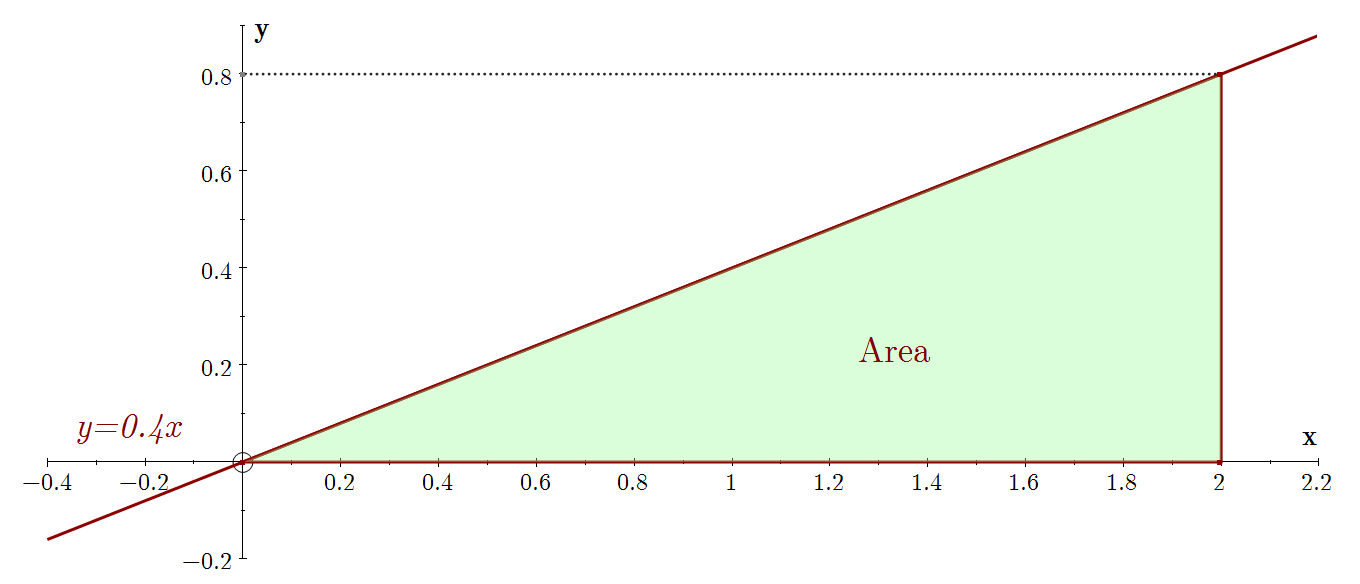
\includegraphics[scale=0.3]{updated/int}
\end{center}
Obviously, $$A=\frac{1}{2}\cdot 2 \cdot 0.8 = 0.8 \ \text{units}^{2}$$ Granted, the following method is very unnecessary (and this problem doesn't even require a multiple integral), but for the sake of explanation, let's employ multiple integrals as well.
\begin{gather*}
A = \underbrace{\int\limits_{0}^{2}}_{\text{(against } x\text{)}} \underbrace{\int\limits_{0}^{0.4x}}_{\text{(against } y\text{)}} \mathrm{d}x \mathrm{d}y =  \int\limits_{0}^{2} \mathrm{d}x \cdot \left[ y \right]_{0}^{0.4x} =  \int\limits_{0}^{2} \mathrm{d}x \cdot  \left[ 0.4x - 0 \right] = \int\limits_{0}^{2} \mathrm{d}x \cdot 0.4x = 0.4 \int\limits_{0}^{2} x\mathrm{d}x = \\
0.4 \cdot \left[ \frac{x^{2}}{2} \right]_{0}^{2} = 0.4 \cdot \left[ \frac{2^{2}}{2} - \frac{0^{2}}{2} \right] = 0.4 \cdot 2 = 0.8.
\end{gather*}
And, again, the answer is the same.
\subsection{Lebesgue Measure} \label{measure}
In mathematical analysis, a measure on a set, is the assignment of a number to all suitable sub-sets of that set.\footnote{\cite{cortzen_weisstein}} Essentially, a measure of a set can be interpreted as its size, and is therefore a generalization of length, area and volume. In particular, the Lebesgue measure assigns length, area and volume (in a conventional sense) to suitable sub-sets of an $m$-dimensional euclidean space $\boldsymbol{R}^m$.\footnote{\cite{lebesgue_1902}} This is particularly useful when dealing with any set that is in more than tree dimensions, as just 'volume' of such a set can not be defined. Thus, a more general idea of 'volume' is used: the Lebesgue Measure.\\
\\
If there is a set $K$ in $\boldsymbol{R}^m$, then the Lebesgue measure of $K$ will be denoted as $\mu(K)$. For example, if $K$ is in $\boldsymbol{R}^1$, and is the interval $[0,1]$, its Lebesgue measure $\mu([0,1])$ is its length, i.e. 1. Similarly, if $K$ is in $\boldsymbol{R}^3$, and is a cube with sides 2, its Lebesgue measure $\mu(K)$ is its volume, i.e. $2^3$ or 8. This principal may be applied to any set in $\boldsymbol{R}^m$ euclidean space.

\section{Formulation of the Problem} \label{formulation}

A function is one of the most known mathematical notions. An important task which has practical applications, is the approximation of a function or relationship based on some information known about the function or relationship in question. This information may either be determinate or statistical. An example of a determinate piece of information about function $f(x)$ is its range (or the possible values this function may have) on a given interval $[\alpha,\beta]$. Example of a statistical information may be the law of distribution of random errors $\xi_{i}$ in approximate values $\tilde{y}_{i} = f(x_{i})+\xi_{i}$ of the function, which in turn can describe a certain physical process (change of temperature over time, for example). In practice,  $n$ number of points $x_{i}$ can be obtained as results of some kind of physical experiment. Where in this case, the approximation of function $f(x)$ only makes sense if this function is described by a finite number $m<n$ of parameters (coefficients) $c_{j}$, where the true values of said parameters will be denoted as $\dot{c}_{j}, \ j=1,2,\dots,m.$ For the sake of convenience, these parameters will be written as an $m$-dimensional vector; $\vecc$ storing the possible parameters and $\dot{\vecc}$ storing the true parameters. \\
\\
This Internal Assessment will focus on the estimation of the parameters of a function 
\usetagform{fn}
\begin{equation} 
y = f(\dot{\vecc},x),\quad \dot{\vecc} \in \boldsymbol{R}^{m},\quad x \in [\alpha,\beta],\quad \dot{\vecc} = (\dot{c}_{1}, \dot{c}_{2},\dots,\dot{c}_{m}) \label{301}
\end{equation}
\footnotetext{Here, because the vector $\dot{\vecc}$ has $m$ parameters (components), it will also be in $m$-dimensional space.}
based on its approximate (i.e containing error) values
\usetagform{default}
\begin{equation}
\tilde{y}_{i} = f(x_{i})+\xi_{i}, \quad i=1,2,\dots,n ,
\end{equation}
when additionally it is also known, that: (1) vector $\dot{\vecc} = (\dot{c}_{1}, \dot{c}_{2},\dots,\dot{c}_{m})$ belongs to a given limited set $D$, like for example a parallelotope\footnote{In geometry, a parallelepiped is a polyhedron in $\boldsymbol{R}^3$, with six faces, each being a parallelogram. It can be generalized to be in $\boldsymbol{R}^m$, then it would take on the name of Parallelotope (\cite{coxeter_1973}). I specifically refer to a Parallelotope as both any cube and any cuboid in $\boldsymbol{R}^m$ is just a special case of a Parallelotope, therefore the term Parallelotope is more general and more accurate in this context. To clarify, a Parallelotope in $\boldsymbol{R}^{3}$ is by definition a parallelepiped.} in $\boldsymbol{R}^{m}$; (2) $\xi$ is a limited continuous random value; the median of which $(Med(\xi))$ is equal to zero. \\
\\
Judging by references in scientific works that I read while researching for this exploration, the most popular linear model of a studied relationship is
\begin{equation}
f(\dot{\vecc},x)= \sum\limits_{j=1}^{m} \dot{\vecc}_{j} \phi_{j}(x), \label{functionform}
\end{equation}
specifically in polynomial form, when
\begin{equation}
\phi_{j}(x)=x^{j-1},\quad j=1,2,\dots,m; \quad \phi_{1}(x) = 1.
\end{equation}
%\\
%In practice, it is often the case when it is not only necessary to estimate the parameters of a function, but identifying the type (structure) of this function is needed as well. In other words, a finite number $L$ of alternative structures is given
%\begin{equation}
%f_{l}(c;x), c \in \boldsymbol{R}^{m(l)}, \quad l=1,2,\dots,L,
%\end{equation}
%and it is necessary to identify to which of $L$ structures of function $f_{l}(c;x)$ belongs the function $f(\dot{c},x)$, and after that estimate the vector $\dot{c}$ of its parameters. In our school program, the class has encountered one such task, when it was said to find out if we were dealing with a linear or exponential relationship, be it in either physics or math. However, then, this problem was solved using the exact (or near to exact) values of both of the relationships, so it was easy to distinguish them. \\
%\\
There are countless papers dedicated to the approximation of functions based on their approximate values (in practice - experimental data). Usually, in such papers the consensus is to use a certain condition. This condition is to assume that the mathematical expectancy of error is equal to zero \footnote{\cite{Plackett_1950}}.
\begin{equation}
E(\xi)=0
\end{equation}
 However, in this exploration this condition will not be used. Here, instead of the condition of mathematical expectancy of error $\xi$ being equal to zero, I will assume that the median of the same error $\xi$ being equal to zero, 
\begin{equation}
Med(\xi)=0
\end{equation}
specifically when the approximation method of the parameters of the function is based on ideas of the \textit{LSM}. \\
\\
In a measurement containing an error $\xi$, that error $\xi$ is considered positive if the measurement itself differs from the true function (like \vref{301}) by a positive value, and negative if that measurement differs by a negative value. I justify my interest to the condition $Med(\xi)=0$ by the case when the traditional condition $E(\xi)=0$ is unachievable. This happens when measurements are taken close to one of the natural limits of the physical relationship being measured. An example of such natural limit is the inability of some magnitude, such as weight, to be negative. In this case, large errors $\xi$ (relative to others) may only occur in such errors $\xi$ that have the same sign, either positive or negative, i.e. in a given case, only positive errors $\xi$ are large or only negative errors $\xi$ are large, depending on the natural limit. Figure \ref{fig:graph-nl} shows an example of this graphically. Here the natural limit is 0 (measurements can not be negative), so large errors $\xi$ only occur while they're positive.
\begin{figure}[h!]
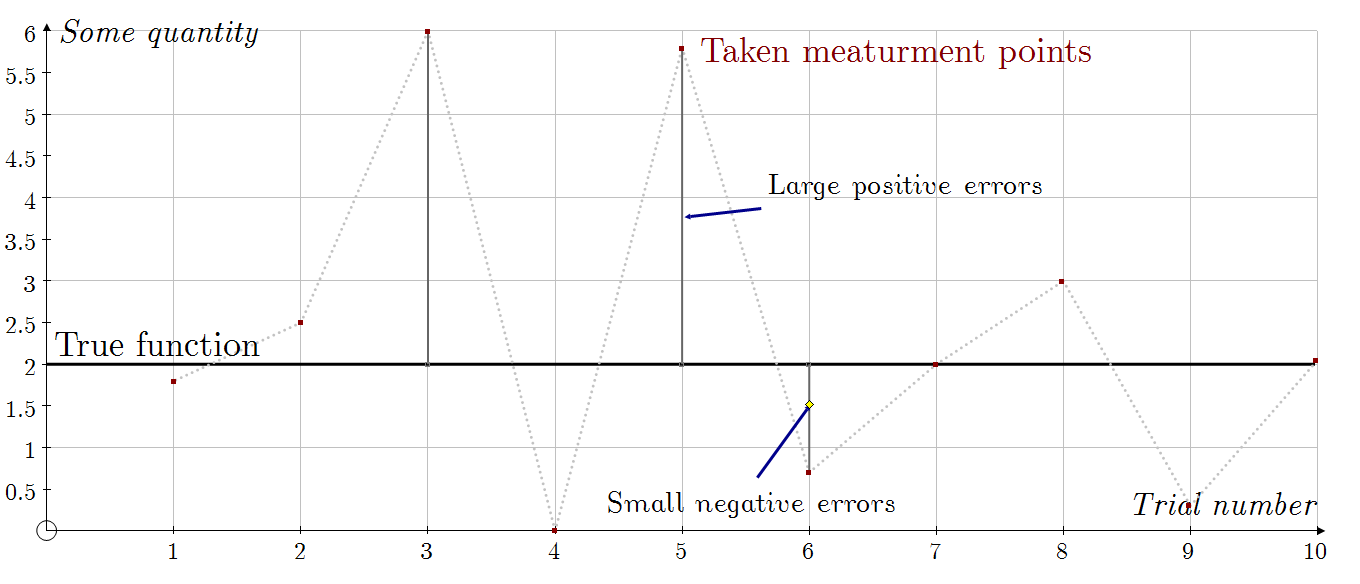
\includegraphics[scale=0.35]{updated/fig1}
\centering
\caption{Graphical representation of a case where $E(\xi)=0$ does not work effectively.}
\label{fig:graph-nl}
\end{figure}
\\
I want to bring attention to the fact, that the argument that this kind of measurement could be withdrawn by human intervention, is invalid for 2 reasons: (1) Any such withdrawal usually leads to loss of information. (2) In cases where the experiment requires high-capacity data collection human intervention may not be possible.\\
\\
What is meant is not only error that was produced by a faulty measurement, but also any error caused by some factor that was either omitted or unaccounted for in function $f(x)$. Even though both conditions $E(\xi)=0$ and $Med(\xi)=0$ are not special cases of each other, it could be argued that from a point of view of solving practical problems, the condition $Med(\xi)=0$ is the more broad of the two (as in, it is easier to meet). The only requirement for meeting this condition is that the probability of $\xi$ being positive is 50\%.  Hence the condition $Med(\xi)=0$ allows for some comparatively large random values of error $\xi$ to be on one side of the true function and not on the other, without the approximation to be significantly affected by those large values, unlike the condition $E(\xi)=0$. With condition $Med(\xi)=0$ the approximation can account for large peaks in values of $\xi$.\\
\\
As mentioned before, the aim of this exploration is to create an algorithm, capable of estimating the parameters of a functional dependence whose structure is known, accurately,  and to securely give an estimate to the accuracy of the calculated approximate values of the functional dependence. \\
\\
Its clear that the quality of the solution of this problem is dependant of an array of factors, which include: (1) the ratio between the $n$ number of measurements $\tilde{y}_{i}$ and the $m$ number of estimated parameters $c_{j}$. (2) the intensity of error $\xi_{i}$. This means that to confirm my theoretical reasoning, quite an ambitions computational experiment is required. I will proceed with the necessary calculations using custom software. 

\section{Algorithm}

Approximation of a functional dependence taking this new condition $Med(\xi)=0$ in mind, has been looked at in mathematics.\footnote{\cite{balk_2010}} It is believed that in this case it is necessary to minimize the sum of absolute values of deviations of the modelled dependence $f(\vecc^{*},x)$ from the unknown true function $f(\dot{\vecc},x)$, where $\vecc^{*}$ is the found optimal value of  vector $\vecc$. This method is referred to as the Least Absolute Deviations (LAD). However, through my research I have found no methods of estimating LAD's accuracy. What value does an optimization method have if there is no way to determining the error it made? In addition, LAD does not presume the existence of priori limitations on the vector $\dot{\vecc}$. And I must ask the question: What happens if the vector of parameters $\vecc^{*}$, providing the minimum of the sum of modulus of errors, does not belong to the set $D$? \\
\\
It is clear, that in any separately taken case (run of an algorithm), the factual accuracy of the model solution (when the true function is known) cannot serve as either a comparative evaluation of two competing algorithms, nor criteria of effectiveness of any given algorithm. This is beacuse the intention of the algorithm itself is to be accurete in practice, i.e. when the true functionn is not known. One separately taken case when compared to the true function may give a good result however there is no way to tell if that result was accedental to that one separatly taken case. It is also clear, that if all, or close to all errors $\xi_{i}$ have the same sign (the condition $Med(\xi)=0$, although, the condition $E(\xi)=0$ as well, allow this, be it with a small probability), then neither method will give any good solutions. So, when estimating the effectiveness of a method, it is necessary to rely on average results of some number of random solutions. In conjunction with this, I will take as a measure of accuracy of constructed approximation $f(\vecc^{*},x)$ to the true function $f(\dot{\vecc},x)$, the mathematical expectation\footnote{\cite{Ross_2007}}

\usetagform{fn}
\begin{equation}
E(\rho(\vecc^{*},\dot{\vecc}))= \int\limits_{D}P(\vecc)\rho(\vecc^{*},\dot{\vecc})\mathrm{d}c_{1}\mathrm{d}c_{2}\dots \mathrm{d}c_{m}, \quad \vecc = (c_{1},c_{2},\dots,c_{m}) \label{Erho}
\end{equation}
\footnotetext{\cite{balk_2010}}
of proximity (distance) $\rho(\vecc^{*},\dot{\vecc})$ of function $f(\vecc^{*},x)$ from $f(\dot{\vecc},x)$ where in the role of distance $\rho(\vecc^{*},\dot{\vecc})$, one could take on of the functions
\usetagform{default}
\begin{eqnarray}
\rho_{1}(\vecc^{*},\vecc) &=& \sum\limits_{j=1}^{m} \left| c{j}^{*}-c_{j} \right| \label{rho1} \qquad \text{( taken from LAD )}\\
\rho_{2}(\vecc^{*},\vecc) &=& \sum\limits_{j=1}^{m} \left( c_{j}^{*}-c_{j} \right)^{2} \label{rho2} \qquad \text{( taken from LSM ).}
\end{eqnarray}
During my research I've found that formula (\vref{Erho}~) was considered in the article \textit{'Reggression-type Problems under Zero Median Noise'} by Peter Balk (referenced earlier as \citep{balk_2010}). There, Balk used a proximity function that is not considered in this exploration. The reason for me using the proximity functions (\vref{rho1}~) and (\vref{rho2}~) instead of the one used in \citep{balk_2010}, is that I will be comparing the method derived here to the already established methods: LSM and LAD. Using a different proximity function, to the ones in those methods, will lead to faulty results. Looking ahead, I say that I will suggest a more constructive algorithm than the one occurring in \citep{balk_2010}.\\
\\
The probability density function $P(\vecc)$, ($\vecc \in D$ where $\vecc$ is any vector that could be the unknown true vector $\dot{\vecc}$), which appears in the $m$-multiple integral (\vref{Erho}~), can be constructed on the basis of the formula of the binomial distribution of a random value [citation needed]. In fact, let's say: $\vecc \in D$ is one of the vectors which claims that it is the unknown true vector $ \dot{\vecc}$ from function (\vref{functionform}~); $q_{i}$ are the elements of the sequence
\begin{equation}
q_{1}(\vecc)=\tilde{y}_{1}-f(\vecc,x_{1}),\ q_{2}(\vecc)=\tilde{y}_{2}-f(\vecc,x_{2}), \dots, \ q_{n}(\vecc)=\tilde{y}_{n}-f(\vecc,x_{n}); \label{sequence}
\end{equation}
where $q$ is a discreet random value, that can assume values
\begin{equation}
r=r(\vecc)=\sum\limits_{i=1}^{n-1} \delta_{i}(\vecc), \label{eq-values-of-q}
\end{equation}
where
\begin{equation}
\delta_{i}=\delta_{i}(\vecc)=
\begin{cases} 
      1, \mathrm{if} \quad q_{i}(\vecc)q_{i+1}(\vecc)<0\\
      0, \mathrm{if} \quad q_{i}(\vecc)q_{i+1}(\vecc)\geq 0
   \end{cases}
\end{equation}
In meaningful terms, $\delta_{i}$ is either 0 or 1 depending on if there has been a transition of sign between two consecutive elements of the sequence (\vref{eq-values-of-q}~). (If the product of those two elements is negative, then one of those elements is negative; hence the transition of sign). Then the value of $r$ is the number of transitions of sign of the elements of  (\vref{sequence}~) where $r \in [0,n-1]$. If it truly happens that $\vecc=\dot{\vecc}$ (the case that is being looked for), then the values of $q_{i}$ would be nothing but the errors $\xi_{i}$, and by the condition $Med(\xi)=0$ the probabilities $p_{r}$ of  $r$ transitions of sign could be written as
\usetagform{fn}
\begin{equation}
p_{r}= \frac{\binom {n-1}r}{2^{n-1}}, \quad r = 0,1,\dots,n-1. \label{priori}
\end{equation}
\footnotetext{\citep{balk_2010}}
Lets move on from discussing the question of the transition of sign with some one vector $\vecc$, to the analysis of this situation with regards to the whole set $D$. Say that there exists a partitioning (splitting) of set $D$ into a family of sub-sets $D_{1},D_{2},\dots,D_{n}$ such that the elements (in this case vectors $\vecc$) of sub-set $D_{r}$ provide the same number  of transitions of sign $r-1$ of elements of (\vref{sequence}~). Note that here the sub-sets $D_{r}$ will take the form of $m$-dimensional polyhedrons \footnote{In geometry, a polyhedron is a solid in three (in this case $m$) dimensions with flat polygonal faces, straight edges and sharp vertices. A polyhedron is said to be convex, if any two points within it can be connected by a line segment with this segment also being within the polyhedron. \cite{cromwell_1999}} as they are in $\boldsymbol{R}^{m}$. In this way, the \textit{a priori} probability\footnote{An a priori probability is a probability that is derived purely by deductive reasoning. \cite{mood_graybill_boes_1974}} that the unknown true vector $\dot{\vecc} \in D_{r}$ in given by (\vref{priori}~). However, in any separate case, some of the sub-sets $D_{r}$ could be empty, meaning  that with some vectors of parameters $\vecc \in D$, the number of transitions of sign of (\vref{sequence}~) will not equal the given value of $r$ (any one can make sure of this by trying to draw a line which would crossed a given poly-line by guess, in such way that all of the endpoints of this poly-line turned out to be on either side of the guessed line). The a priori probabilities $p_{r}$ that the unknown true vector $\dot{\vecc}$ is in one of the non-empty sub-sets $D_{r}$ can be recalculated to the \textit{posteriori} probabilities\footnote{The posteriori probabilities of an event is the ratio of the number of outcomes in which a specified event occurs to the total number of trials, not in a theoretical sample space but in an actual experiment. In a more general sense, empirical probability estimates probabilities from experience and observation.\cite{mood_graybill_boes_1974}} $p_{r}^{*}$. Let's define $I$ as the set of the numbers of all the non-empty sub-sets $D_{r}$. Then
\usetagform{default}
\begin{equation}
p_{r}^{*}= 
\begin{cases} 
		\frac{p_{r}}{\sum\limits_{s \in I}p_{s}}, \quad r \in I.\\
		0, \quad r \in \{ 0,1,\dots,n-1 \} \setminus I.
\end{cases} \label{posteriori}
\end{equation}
To clarify, here the a priori probabilities suggested a chance that the true vector $\dot{\vecc}$ could be in sub-sets $D_{r}$ which are empty. This is obviously not possible. The equation (\vref{posteriori}~) nullifies those cases, and redistributes those probabilities proportionally across the experimentally possible cases.\\
\\
Because in our case the vectors $\vecc$, are continuous values, and not discreet ones, then to use formula (\vref{Erho}~) we must proceed from estimates $p_{r}^{*}$ of the probabilities of event $\dot{\vecc} \in D_{r}$ to estimates $p_{r}^{*}(\vecc), \vecc \in D_{r}$, of a probability density function. As there is no information suggesting the distribution of vectors $\vecc$ in the bounds of each sub-set $D_{r}$, it is logical to assume uniform distribution across each sub-set. Then for all $r \in I$
\begin{equation}
P_{r}^{*}(\vecc)=\frac{p_{r}^{*}}{\mu(D_{r})}, \quad \vecc \in D_{r} \label{posteriori}
\end{equation}
where $\mu(D_{r})$ is the Lebesgue measure (explained in section \vref{measure}) of sub-set $D_{r}$ in $\boldsymbol{R}^{m}$. \\
\\
Therefore (\vref{Erho}~) becomes
\begin{gather}
E(\rho(\vecc^{*},\dot{\vecc}))=\sum\limits_{r \in I} \frac{p_{r}^{*}(\vecc)}{\mu(D_{r})} \int\limits_{D_{r}}\rho(\vecc^{*},\dot{\vecc})\mathrm{d}c_{1}\mathrm{d}c_{2}\dots \mathrm{d}c_{m} \label{mathexpectancy}\\
\nonumber
\text{( where $\int_ {D_{r}}(\bullet)$ is a laconic notation of an $m$-multiple integral )}
\end{gather}
In the general case, such as this one, the limits of integration of each univariate integral depend on other variables, based on which the integration of the external integral relative to the given univariate integral is carried out.\footnote{\cite{stewart_2008_int}} (Refer to the example in section \vref{multiint}). This significantly complicates the calculation of these multiple integrals. Yet again, looking ahead, I want to note that in the algorithm created, integration is carried out on multidimensional parallelepipeds, when the limits of integration of each integral remain constant.

\subsection{Illustrative example}
Let's consider an illustrative example. Here, I will be comparing my method to the LSM. In this example $m=1$ (i.e. the vector $\dot{\vecc}$ can be treated as a scalar value), $y=f(\vecc;x)$ is a function with one parameter, where $\dot{\vecc}$ is a vector that has to be found. Let $n=6$ and $D=\{ \vecc: 2 \leq \vecc \leq 6 \}$.
%\begin{figure}[h!]%
%    \centering
%    \subfloat[Graph of proposed example]{{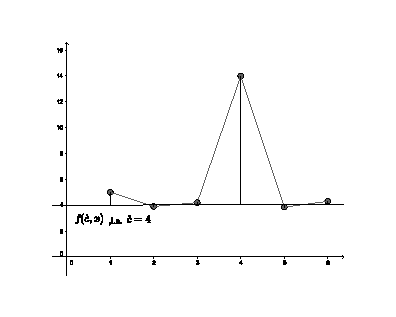
\includegraphics[height=7cm]{IlusExample} }}%
%    \qquad
%    \subfloat[Illustration of transitions of sign $q_{i}$ between each $\tilde{y}_{i}$]{{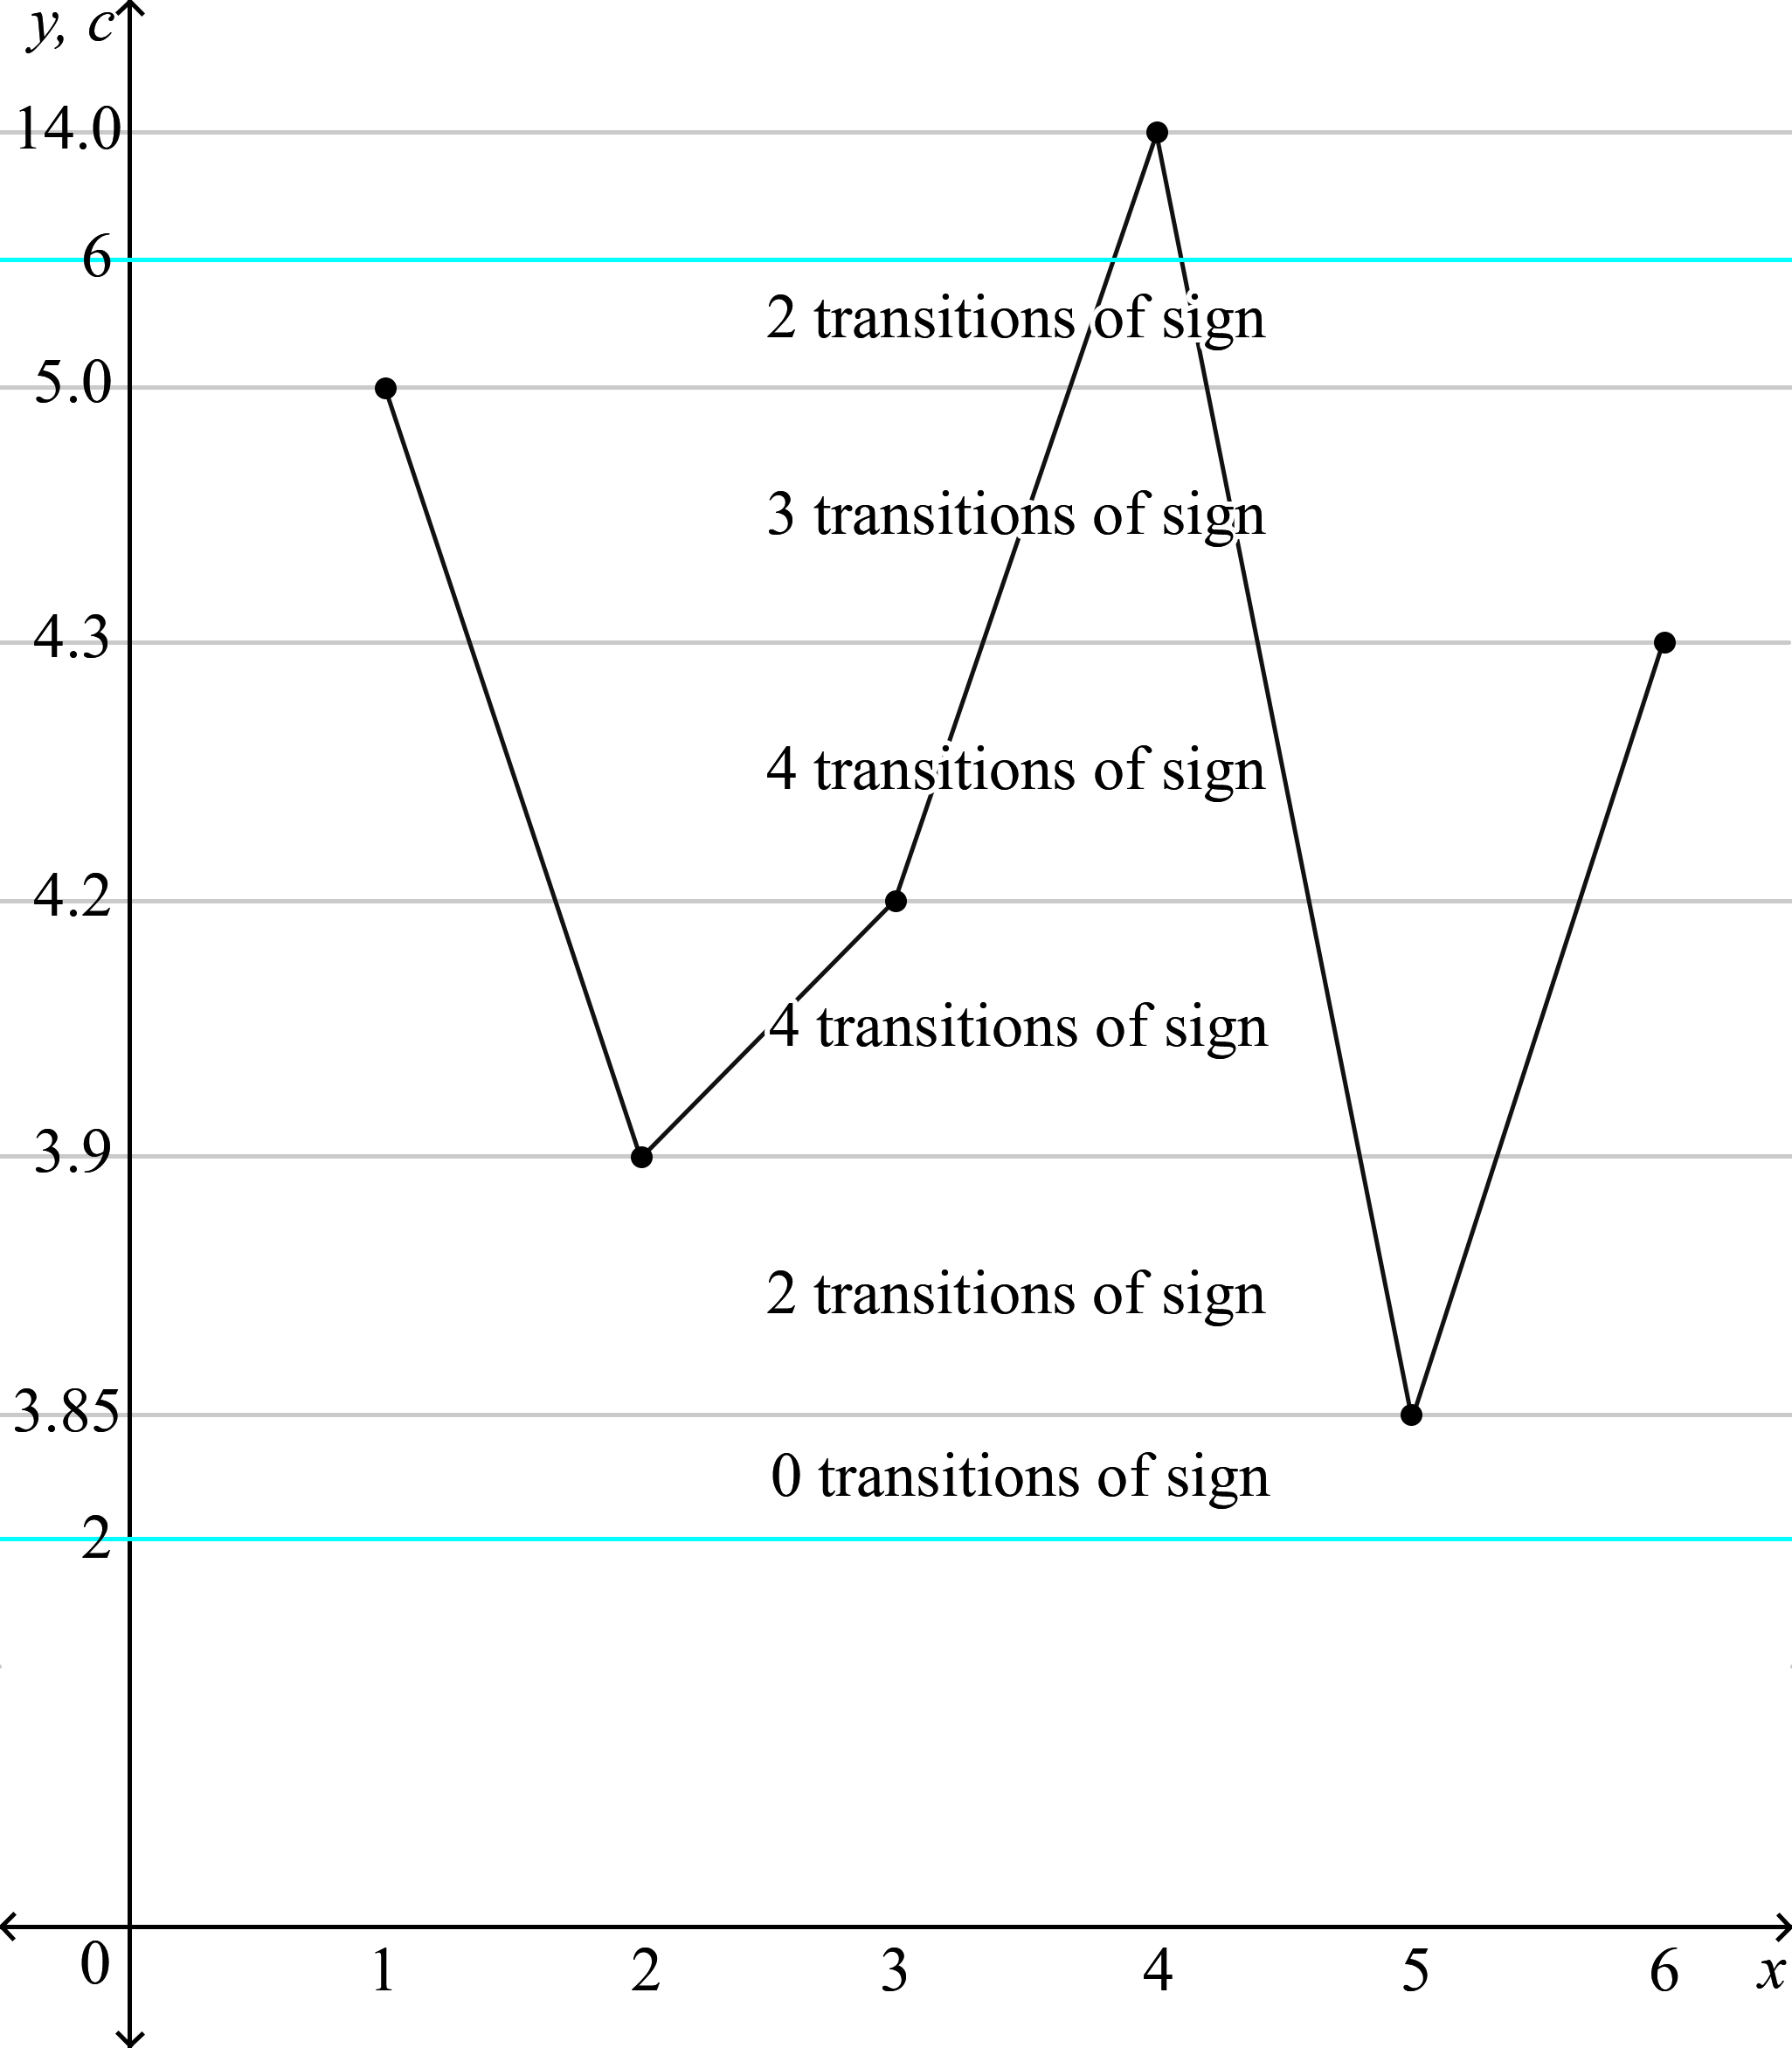
\includegraphics[height=6cm]{examplegraph} }}
%    \caption{ }%
%    \label{fig:example}%
%\end{figure}

\begin{table}[h!]
\caption {Table of values for this example} \label{tab:title} 
\centering
\begin{tabular}{lllll}
$i$ & $x_{i}$ & $f(\dot{\vecc},x_{i})$ & $\xi_{i}$  & $\tilde{y}_{i}=f(\dot{\vecc},x_{i})+\xi_{i}$  \\
1 & 1 & 4      & 1.0   & 5.0   \\
2 & 2 & 4      & -0.1  & 3.9   \\
3 & 3 & 4      & 0.2   & 4.2   \\
4 & 4 & 4      & 10    & 14.0  \\
5 & 5 & 4      & -0.15 & 3.85  \\
6 & 6 & 4      & 0.3   & 4.3  
\end{tabular}
\end{table}
\noindent
For this example I will use proximity function (\vref{rho2}~) also used in LSM. I am doing this as I will later compare the two methods.\\
\noindent
As we already know, we can calculate the a priori probabilities using (\vref{priori}~), where $r=0,1,2,3,4,5$ like so:
\begin{gather*}
p_{0}= \frac{1}{32}; \ p_{1}= \frac{5}{32}; \ p_{2}= \frac{10}{32}; \ p_{3}= \frac{10}{32}; \ p_{4}= \frac{5}{32}; \ p_{5}= \frac{1}{32}
\end{gather*}
But in this case there can only be certain values of $r$, namely the values of set $I=\{0,2,3,4\}$. (This is because in this example there is no possible vector $\vecc$ that would produce a line that would give either 1 or 5 transitions of sign). And ,so 
\begin{gather*}
\sum\limits_{s \in I}p_{s}=p_{0}+p_{2}+p_{3}+p_{4}= \frac{1}{32} + \frac{10}{32} + \frac{10}{32} + \frac{5}{32} = \frac{26}{32}.
\end{gather*}
So, to calculate the posteriori probabilities using (\vref{posteriori}~)
\begin{eqnarray*}
p_{0}^{*} &=& p_{0}: \frac{26}{32} = \frac{1}{32} : \frac{26}{32} = \frac{1}{26} \\
p_{1}^{*} &=& 0 \\
p_{2}^{*} &=& p_{2}: \frac{26}{32} = \frac{10}{32} : \frac{26}{32} = \frac{10}{26} \\
p_{3}^{*} &=& p_{3}: \frac{26}{32} = \frac{10}{26} \\
p_{4}^{*} &=& p_{4}: \frac{26}{32} = \frac{5}{32} : \frac{26}{32} = \frac{5}{26} \\
p_{5}^{*} &=& 0
\end{eqnarray*}
Calculating $E(\rho(\vecc^{*},\vecc))$
\begin{gather*}
E(\rho(\vecc^{*},\vecc)) = \int\limits_{2}^{3.85} \underbrace{(\vecc^{*}-\vecc)^{2}}_{\rho(\vecc^{*},\vecc)} \cdot \frac{\overbrace{\frac{1}{26}}^{p_{0}^{*}}}{\underbrace{3.85-2}_{\mu(D_{0})}} \mathrm{d}\vecc \ + \int\limits_{3.85}^{3.9} (\vecc^{*}-\vecc)^{2} \cdot \frac{\frac{10}{26}}{1.05} \mathrm{d}\vecc + \int\limits_{3.9}^{4.3} (\vecc^{*}-\vecc)^{2} \cdot \frac{\frac{5}{26}}{4.3-3.9} \mathrm{d}\vecc \\
+ \int\limits_{4.3}^{5.0} (\vecc^{*}-\vecc)^{2} \cdot \frac{\frac{10}{26}}{5.0-4.3} \mathrm{d}\vecc + \int\limits_{5.0}^{6.0} (\vecc^{*}-\vecc)^{2} \cdot \frac{\frac{10}{26}}{1.05}  \mathrm{d}\vecc
\end{gather*}
Taking into account that later we will want to find the derivative $\frac{\mathrm{d}E(\rho(\vecc^{*},\vecc))}{\mathrm{d}\vecc^{*}}$, we can omit the summand $\frac{1}{3} \vecc^{3}$ as it is a constant, and the derivative of a constant is zero. Let's continue.
\begin{eqnarray*}
E(\rho(\vecc^{*},\vecc)) =& 0.021 & \cdot\left[ (\vecc^{*})^{2} \cdot \vecc - \vecc^{*} \cdot \vecc^{2} + \frac{1}{3} \vecc^{3}\right]_{2}^{3.85}  \\
+ & 0.366 &\cdot\left[ (\vecc^{*})^{2} \cdot \vecc - \vecc^{*} \cdot \vecc^{2} + \frac{1}{3} \vecc^{3} \right]_{3.85}^{3.9} \\
+ & 0.481 &\cdot\left[ (\vecc^{*})^{2} \cdot \vecc - \vecc^{*} \cdot \vecc^{2} + \frac{1}{3} \vecc^{3} \right]_{3.9}^{4.3}  \\
+ & 0.549 &\cdot\left[ (\vecc^{*})^{2} \cdot \vecc - \vecc^{*} \cdot \vecc^{2} + \frac{1}{3} \vecc^{3} \right]_{4.3}^{5.0}  \\
+ & 0.366 &\cdot\left[ (\vecc^{*})^{2} \cdot \vecc - \vecc^{*} \cdot \vecc^{2} + \frac{1}{3} \vecc^{3} \right]_{5.0}^{6.0}  \\
= & 1.000 &\cdot(\vecc^{*})^{2}-9.55\vecc^{*} + 23.282
\end{eqnarray*}

\begin{eqnarray*}
\frac{\mathrm{d}E(\rho(\vecc^{*},\vecc))}{\mathrm{d}\vecc^{*}} &=& 2\vecc^{*}-9.55 = 0 \\
\vecc^{*} &=& \frac{9.55}{2} = 4.773
\end{eqnarray*}
Seeing that $\dot{\vecc} = 4.0$, we finally calculate $\rho$ using this method
\begin{equation*}
\rho = |4.773-4.0| = 0.773
\end{equation*}
Error made by this method is 0.431. Now let's see what kind of error will the LSM give:
\begin{eqnarray*}
\text{Using Least Square Method} \\
\phi(\vecc^{*})= \sum\limits_{i=1}^{6}(\tilde{y}_{i}-\vecc^{*})^{2} \longrightarrow min &\qquad & \text{(Sum of the squares of errors has to be minimised)}\\
\phi(\vecc^{*})= \sum\limits_{i=1}^{6}(\tilde{y}_{i}^{2}-2 \tilde{y}_{i}\vecc^{*} + (\vecc^{*})^{2}) &\qquad & \text{(Expanding the polynomial)}\\
\frac{\mathrm{d}\phi(\vecc^{*})}{\mathrm{d}\vecc^{*}} =  \sum\limits_{i=1}^{6}(0 -\cancel{2} \tilde{y}_{i} +\cancel{2} \vecc^{*}) = 0  &\qquad & \text{(Finding the derivative and equating it to zero)}\\
 \sum\limits_{i=1}^{6}\vecc^{*} = \sum\limits_{i=1}^{6} \tilde{y}_{i} &\qquad & \text{(Re-arranging the result)}\\
 6 \cdot \vecc^{*} = \sum\limits_{i=1}^{6} \tilde{y}_{i} = 35.25 &\qquad & \\
 \vecc^{*} = \frac{35.25}{6} = 5.875 &\qquad & \text{(Solving for $\vecc^{*}$)}\\
& \qquad & \text{And so the error } \rho = 1.875
\end{eqnarray*}
LSM gives a bigger error because in it deviations are squared \footnote{\cite{Plackett_1950}}, and therefore large derivations are weighted more heavily. Because this example shows, that in the case of significant non-compliance to condition $E(\xi)=0$, my method is notably superior to LSM, and because of the limited format of this exploration, I will not include further solutions that used LSM. %You may refer to (*) in the apendix for more such results.
 Back to the theory.\\
\\
Let the proximity $\rho(\vecc^{*},\vecc)$ in (\vref{mathexpectancy}~), be taken in the form (\vref{rho2}~). Then the following simplification takes place.
\begin{gather}
\nonumber
E(\rho(\vecc^{*},\dot{\vecc}))=\sum\limits_{r \in I} \frac{p_{r}^{*}}{\mu(D_{r})} \int\limits_{D_{r}}\sum\limits_{j=1}^{m} \left( c_{j}^{*}-c_{j} \right)^{2}\mathrm{d}c_{1}\mathrm{d}c_{2}\dots \mathrm{d}c_{m}\\
\nonumber
\textit{expanding} \left( c_{j}^{*}-c_{j} \right)^{2} \\
\nonumber
=\sum\limits_{r \in I} \frac{p_{r}^{*}}{\mu(D_{r})} \sum\limits_{j=1}^{m} \left[ (c_{j}^{*})^{2} \underbrace{\int\limits_{D_{r}} \mathrm{d}c_{1}\mathrm{d}c_{2}\dots \mathrm{d}c_{m}}_{{=\mu(D_{r})}} - 2c_{j}^{*} \int\limits_{D_{r}} c_{j} \  \mathrm{d}c_{1}\mathrm{d}c_{2}\dots \mathrm{d}c_{m} + \int\limits_{D_{r}} c_{j}^{2} \  \mathrm{d}c_{1}\mathrm{d}c_{2}\dots \mathrm{d}c_{m}\right]\\
\nonumber
=\sum\limits_{j=1}^{m} \left( \sum\limits_{r \in I} \frac{p_{r}^{*}}{\mu(D_{r})} \left[ (c_{j}^{*})^{2} \mu(D_{r})-2c_{j}^{*} \int\limits_{D_{r}} c_{j} \  \mathrm{d}c_{1}\mathrm{d}c_{2}\dots \mathrm{d}c_{m} + \int\limits_{D_{r}} c_{j}^{2} \  \mathrm{d}c_{1}\mathrm{d}c_{2}\dots \mathrm{d}c_{m} \right] \right)\\ 
=\sum\limits_{j=1}^{m} \left( (c_{j}^{*})^{2} \cancel{\mu(D_{r})} \underbrace{\sum\limits_{r \in I} \frac{p_{r}^{*}}{\cancel{\mu(D_{r})}}}_{\sum\limits_{r \in I}p_{r}^{*} = 1} - 2c_{j}^{*} \sum\limits_{r \in I}\frac{p_{r}^{*}}{\mu(D_{r})} \int\limits_{D_{r}} c_{j} \  \mathrm{d}c_{1}\mathrm{d}c_{2}\dots \mathrm{d}c_{m} + \sum\limits_{r \in I}\frac{p_{r}^{*}}{\mu(D_{r})} \int\limits_{D_{r}} c_{j}^{2} \  \mathrm{d}c_{1}\mathrm{d}c_{2}\dots \mathrm{d}c_{m} \right)
\end{gather}
And finally:
\begin{equation}
E(\rho(\vecc^{*},\dot{\vecc}))= \sum\limits_{j=1}^{m} \left( (c_{j}^{*})^{2} - 2c_{j}^{*} \sum\limits_{r \in I} p_{r}^{*} \frac{\int\limits_{D_{r}} c_{j} \  \mathrm{d}c_{1}\mathrm{d}c_{2}\dots \mathrm{d}c_{m}}{\mu(D_{r})} + \underbrace{\sum\limits_{r \in I} p_{r}^{*} \frac{\int\limits_{D_{r}} c_{j}^{2} \  \mathrm{d}c_{1}\mathrm{d}c_{2}\dots \mathrm{d}c_{m}}{\mu(D_{r})}}_{\text{derivative of this with respect to } c_{1}^{*}, c_{2}^{*},\dots,c_{m}^{*} = 0} \right) \label{eq-Erho-simp}
\end{equation}
In order to find the vector $c^{*}$, which provides the minimum of function (\vref{eq-Erho-simp}~) and which I will take as the optimal estimate of the unknown vector $\dot{c}$, it is necessary (like in the case with a simple one-parameter function) to take the first partial derivative $\frac{\partial E}{\partial c_{j}^{*}}$ of function (\vref{eq-Erho-simp}~) with respect to each variable $c_{j}^{*}$ \footnote{\cite{stewart_2008_deriv}}. After that, equate these derivatives to zero and solve the resulting system of linear equations. In this case, this system splits into $m$ separate linear equation with one variable:
\begin{equation}
2 c_{j}^{*} - 2 \sum\limits_{r \in I} p_{r}^{*}\frac{\int\limits_{D_{r}} c_{j}\mathrm{d}c_{1}\mathrm{d}c_{2}\dots\mathrm{d}c_{m}}{\mu(D_{r})} = 0, \quad j = 1,2,\dots,m.
\end{equation}
These equations have the following solutions:
\begin{equation}
c_{j}^{*} = \sum\limits_{r \in I} p_{r}^{*} \bar{c}_{(j,r)}, \quad j = 1,2,\dots,m, \label{eq-solutions-to-cj*}
\end{equation}
where
\begin{equation}
\bar{c}_{(j,r)} = \frac{\int\limits_{D_{r}} c_{j}\mathrm{d}c_{1}\mathrm{d}c_{2}\dots\mathrm{d}c_{m}}{\mu(D_{r})}. \label{eq-cbar}
\end{equation}

\section{Algorithm trials}
Let us look at a model function, the parameters (coefficients) of which will have to be approximated by the method derived in this exploration and the known, conventional methods LAD and LSM. This function $f(\dot{\vecc},x) = \dot{c}_1 + \dot{c}_2x$ has two parameters which will be $\dot{c}_1=2$ and $\dot{c}_2=0.5$ respectively. The approximation of these parameters $\dot{c}_1$ and $\dot{c}_2$ will be carried out from $n=20$ values (containing random errors $\xi_i$) $\tilde{y}_{i} = f(\dot{\vecc},x)+\xi_{i}, \quad i=1,2,\dots,n$. The errors $\xi_i$ are random normally distributed values with mean 0 and standard deviation $\sigma$.\\
\\
Due to a the technical requirement (described in Appendix A: section \vref{apendix}) (and also theoretically explained in section \vref{formulation}) it is also necessary that the true vector $\dot{\vecc}$ be limited to a set $D$. Therefore we define this set $D$ such that
\begin{equation}
\dot{\vecc} =  (\dot{c}_1 ,\dot{c}_2) \in D = \{ (c_1 ,c_2) : \quad 1 \leqslant c_1 \leqslant 3; \quad 0 \leqslant c_2 \leqslant 1 \}.
\end{equation}

\begin{table}[h!]
\centering
\caption{Average results of 5 algorithm trials. Each group of 5 calculated with a increasing standard deviation $\sigma$ of error $\xi_{i}$. Proximity function used (\vref{rho1}~) is taken from LAD in order to compare the derived method with LAD.}
\label{my-label}
\bgroup
\def\arraystretch{1.3}
\begin{tabular}{|c|r|r|r|r|r|r|r|}
\hline
\multirow{2}{*}{\begin{tabular}[c]{@{}c@{}}Intensity\\ of error\end{tabular}} & \multicolumn{4}{c|}{My method}                                                                                                                                                                                                     & \multicolumn{3}{c|}{LAD}                                                                                                                           \\ \cline{2-8} 
                                                                              & \multicolumn{1}{c|}{$c_{1}^{*}$} & \multicolumn{1}{c|}{$c_{2}^{*}$} & \multicolumn{1}{c|}{\begin{tabular}[c]{@{}c@{}}Expected\\ error\end{tabular}} & \multicolumn{1}{c|}{\begin{tabular}[c]{@{}c@{}}Factual\\ error\end{tabular}} & \multicolumn{1}{c|}{$c_{1}^{*}$} & \multicolumn{1}{c|}{$c_{2}^{*}$} & \multicolumn{1}{c|}{\begin{tabular}[c]{@{}c@{}}Factual\\ error\end{tabular}} \\ \hline
$\sigma = 0.1$                                                                & 2.027                            & 0.497                            & 0.269                                                                         & 0.192                                                                        & 2.051                            & 0.459                            & 0.100                                                                        \\ \cline{1-1}
$\sigma = 0.3$                                                                & 2.049                            & 0.517                            & 0.468                                                                         & 0.302                                                                        & 2.146                            & 0.388                            & 0.288                                                                        \\ \cline{1-1}
$\sigma = 1.0$                                                                & 2.218                            & 0.459                            & 0.655                                                                         & 0.354                                                                        & 2.411                            & 0.297                            & 0.697                                                                        \\ \hline
\end{tabular}
\egroup
\end{table}

\begin{table}[!h]
\centering
\caption{One algorithm run with 5 trials (each trial has randomized errors $\xi_{i}$). Proximity function used (\vref{rho2}~) is taken from LSM in order to compare the derived method to LSM.}
\bgroup
\def\arraystretch{1.3}
\begin{tabular}{|c|r|r|r|r|r|r|r|}
\hline
\multirow{2}{*}{Trial} & \multicolumn{4}{c|}{My method}                                                                                                                                                                                                     & \multicolumn{3}{c|}{LSM}                                                                                                                           \\ \cline{2-8} 
                       & \multicolumn{1}{c|}{$c_{1}^{*}$} & \multicolumn{1}{c|}{$c_{2}^{*}$} & \multicolumn{1}{c|}{\begin{tabular}[c]{@{}c@{}}Expected\\ error\end{tabular}} & \multicolumn{1}{c|}{\begin{tabular}[c]{@{}c@{}}Factual\\ error\end{tabular}} & \multicolumn{1}{c|}{$c_{1}^{*}$} & \multicolumn{1}{c|}{$c_{2}^{*}$} & \multicolumn{1}{c|}{\begin{tabular}[c]{@{}c@{}}Factual\\ error\end{tabular}} \\ \hline
1                      & 2.065                            & 0.404                            & 0.199                                                                         & 0.013                                                                        & 2.593                            & -0.217                           & 0.866                                                                        \\ \cline{1-1}
2                      & 2.136                            & 0.556                            & 0.157                                                                         & 0.021                                                                        & 2.416                            & 0.438                            & 0.177                                                                        \\ \cline{1-1}
3                      & 1.844                            & 0.707                            & 0.161                                                                         & 0.067                                                                        & 2.470                            & 0.223                            & 0.298                                                                        \\ \cline{1-1}
4                      & 2.156                            & 0.495                            & 0.150                                                                         & 0.024                                                                        & 2.693                            & -0.281                           & 1.091                                                                        \\ \cline{1-1}
5                      & 2.156                            & 0.343                            & 0.161                                                                         & 0.049                                                                        & 2.550                            & 0.075                            & 0.483                                                                        \\ \cline{1-1}
Average                & 2.071                            & 0.501                            & 0.165                                                                         & 0.035                                                                        & 2.544                            & 0.047                            & 0.583                                                                        \\ \hline
\end{tabular}
\egroup
\end{table}

\begin{table}[!h]
\centering
\caption{My caption}
\label{my-label}
\bgroup
\def\arraystretch{1.3}
\begin{tabular}{|l|l|l|l|l|}
\hline
Average & $n=6$  & $n=10$ & $n=20$ & $n=30$ \\ \hline
$c_1^*$ & 2.089  & 2.025  & 1.999  & 1.993  \\ \cline{1-1}
$c_2^*$ & 0.3877 & 0.4759 & 0.4816 & 0.4824 \\ \hline
\end{tabular} 
\egroup
\end{table}
\newpage
\section{Conclusion}


\newpage

\section{Appendix A} \label{apendix}
\subsection{Method Description of Computation of Theoretical Algorithm}

Here I will make use of the product notation:
\begin{gather*}
\prod\limits_{i = m}^{n} x_{i} = x_{m} \cdot x_{m+1} \cdot \  \cdots \  \cdot x_{n-1} \cdot x_{n}.
\end{gather*}
This essentially works in much of the same way the familiar summation notation we use in class(using the Greek capital letter sigma), except that instead of summing values, it multiplies them (and uses Greek capital letter pi).\footnote{\cite{product_1995}}\\
\\
From the point of view of practical realisation of my algorithm, that is based of formulae (\vref{eq-solutions-to-cj*}~),(\vref{eq-cbar}~), I can ask two questions: (1) Is it possible to derive a simple method of constructing the sets $D_{r}$? (2) Is it possible to derive a simple method of calculation the integrals of those sets $D_{r}$, which appear in the RHS of (\vref{eq-cbar}~). What a geometrical construction (Figure omitted) has shown me, is that even in the case where $m=2$ and $n=10$, the regions $D_{r}$ have a relatively complicated geometry (some multi-peaked star-like shapes). However, this problem can be solved with the principal of the 'Gordian knot' - refuse to work with directly with sets $D_{r}$, but instead, to use their point (grid) approximation (even without describing these sets concretely) and use an analog of (\vref{eq-solutions-to-cj*}~).\\
\\
The essence of this suggested method of thinking is as follows. Define $k(1),k(2),\dots,k(m)$ as some quite large real values, and a $m$-dimensional parallelepiped
\begin{equation}
W=\{ c:c_{j}^{(\text{min)}} \leq c_{j} \leq c_{j}^{(\text{max)}}, \quad j=1,2,\dots,m \}\subset \boldsymbol{R}^{m}
\end{equation}
which contains the set $D$ (if the set $D$ itself is a parallelepiped, then $W=D$). Cover this parallelepiped with a dense grid $\Gamma$ with
\begin{equation}
L = \prod\limits_{t=1}^{m}k(t)
\end{equation}
number of nodes $\vecc^{(l)} = (c_{1}^{(l)},(c_{2}^{(l)},\dots,c_{m}^{(l)}),\quad l=1,2,\dots,L$, where each coordinate $c_{j}^{(l)}, \quad j=1,2,\dots,m,$ could independently from all the other $m-1$ coordinates (note that $m-1$ does not refer to sets of coordinates) assume one of $k(j)$ of values
\begin{equation}
c_{j}=c_{j}^{(\text{min})} + \frac{c_{j}^{(\text{max})}-c_{j}^{(\text{min})}}{k(j)}(t-\frac{1}{2}), \quad t=1,2,\dots,k(j).
\end{equation}
Parallel to grid $\Gamma$ implement the system $A$ of parallelepipeds $W_{l} \subset \boldsymbol{R}^{m}, \quad l=1,2,\dots,L,$ the centres of which are their nodes with sides
\begin{gather}
h_{j} = \frac{(c_{j}^{(\text{max})}-c_{j}^{(\text{min})})}{k(j)}: \\
W_{l} = \lbrace \vecc=(c_{1},c_{2},\dots,c_{m}):c_{j}^{(l)}-\frac{1}{2} h_{j} \leq c_{j} \leq c_{j}^{(l)}+\frac{1}{2} h_{j}, \quad j=1,2,\dots,m \rbrace .
\end{gather}
These parallelepipeds form the surface of the parallelepiped W. Now we have to chose from the defined $L$ nodes those, the ones who belong to the set $D$. Let $L_{0}$ be the quantity of the chosen nodes. Renumber the chosen nodes, by assigning the first $L_{0}$ numbers $l$ to them. \\
\\
For each $l=1,2,\dots,L_{0}$ find elements of $q_{i}(c^{(l)}), \quad i=1,2,\dots,n$ of sequence (\vref{sequence}~), and based on their values, using (\vref{eq-values-of-q}~), calculate the number $r$ of transition of sign of elements of (\vref{sequence}~). Let $J_{r}, \quad r=0,1,\dots,n-1$ be the set of numbers $l$ of chosen nodes $c^{(l)}$ providing $r$ transitions of sign, and $|J_{r}|$ - the number of nodes giving that many transitions. In this way, without directly constructing the sub-sets $D_{r}$, I approximate each of them with the union.\footnote{\cite{smith_eggen_andre_2015}}
\begin{equation}
\tilde{D}_{r} = \bigcup_{l \in J_{r}} W_{l}. \tag*{(\theequation)\protect\footnotemark}
\end{equation}
\footnotetext{Here, $\tilde{D_{r}}$ is the arbitrary union of all sets $W_l$ such that $l$ is an element of $J_r$.}
\\
It is clear, that the assumption, that all vectors $\vecc$, belonging to the parallelepiped $W_{l}$, will provide the same number of transitions of sign as the center $\vecc^{(l)}$ of the parallelepiped, will only be incorrect for those parallelepipeds $W_{l}$, and do not completely belong to some one sub-set $D_{r}$. But with a dense grid $\Gamma$, and respectively, quite small-sized parallelepipeds $W_{l}$, the percent of such 'debatable' parallelepipeds compared to their general number $L_{0}$ will be quite small (so, in figure (omitted), when $m=2$, these 'debatable' parallelepipeds are positioned along the lines, and the 'non-debatable' - in the areas). In addition, the error resulting from classification of such 'debatable' parallelepipeds $W_{l}$ completely to some set $D_{r}$, will get (mostly) redeemed/repaid. Summing up all these arguments, it can be said, that the approximations of sets $D_{r}$, with the union of relatively 'small' parallelepipeds will give a good  approximation of the mathematical expectancy (\vref{mathexpectancy}~) of error in estimation of parameters of a studies functional dependence:
\begin{gather}
\nonumber
E(\rho_{2}(\vecc^{*},\vecc)) \approx \sum\limits_{r \in I} \frac{p_{r}^{*}}{\mu(\tilde{D}_{r})} \int\limits_{\tilde{D}_{r}} \sum\limits_{j=1}^{m}(c_{j}^{*}-c_{j})^{2}\mathrm{d}c_{1}\mathrm{d}c_{2}\dots \mathrm{d}c_{m} = \\
\nonumber 
\text{(integral with limit } D_{r} \text{ can be split as the sum of integrals with limit } W_{l} \text{)}\\
\sum\limits_{r \in I} \frac{p_{r}^{*}}{\mu(\tilde{D}_{r})} \sum\limits_{l \in J_{r}} \  \int\limits_{W_{l}} \sum\limits_{j=1}^{m}(c_{j}^{*}-c_{j})^{2}\mathrm{d}c_{1}\mathrm{d}c_{2}\dots \mathrm{d}c_{m} = \\
\nonumber
\text{(the sum } \sum_{j=1}^{m} \text{ is facrotised out)} \\
\nonumber
\sum\limits_{j=1}^{m}  \left[ \sum\limits_{r \in I} \frac{p_{r}^{*}}{\mu(\tilde{D}_{r})} \left( \sum\limits_{l \in J_{r}} \ \int\limits_{W_{l}} ((c_{j}^{*})^{2}-2c_{j}^{*}c_{j}+c_{j}^{2}) \right) \mathrm{d}c_{1}\mathrm{d}c_{2}\dots \mathrm{d}c_{m} \right] = \\
\nonumber
\text{(expanding } ((c_{j}^{*})^{2}-2c_{j}^{*}c_{j}+c_{j}^{2}) \text{)}\\
\sum\limits_{j=1}^{m}  \left[ \sum\limits_{r \in I} \frac{p_{r}^{*}}{\mu(\tilde{D}_{r})} \left( \sum\limits_{l \in J_{r}} \left[ (c_{j}^{*})^{2} \mu(W_{(l)}) - 2c_{j}^{*} \int\limits_{W_{l}} c_{j} \mathrm{d}c_{1}\mathrm{d}c_{2}\dots \mathrm{d}c_{m} + \int\limits_{W_{l}} c_{j}^{2} \mathrm{d}c_{1}\mathrm{d}c_{2}\dots \mathrm{d}c_{m} \right] \right) \right]. \label{eq-simplification-chain}
\end{gather}
If in a multiple integral, the limits of integration for each variable are given by other variables, then this multiple integral is equal to the product of included in it, one-dimensional integrals \footnote{\cite{stewart_2008_int}}. Now, if we define coordinates of the edges of $W_{l}$ as $c_{j}^{(l)} - 0.5h_{j} = a(j,l)$ and $c_{j}^{(l)} + 0.5h_{j} = b(j,l)$ then it is not hard to be sure that 
\begin{equation}
\frac{1}{\mu(W_{l})} \int\limits_{W_l} c_{j} \mathrm{d} c_{1} \mathrm{d} c_{2} \ldots  \mathrm{d} c_{m} 
	= \dfrac{1}{\prod\limits_{s=1}^{m}h_{s}}
	\left( \  \int\limits_{b(j,l)}^{a(j,l)} c_{j}  \mathrm{d} c_{j}\right) 
	\prod_{\substack{s=1\\ (s\ne j)}}^m \ 
	\int\limits_{a(s,l)}^{b(s,l)} \!  \mathrm{d} c_{s} 
	= c_{j}^{(l)}.
\end{equation}
If in addition we accept that
\begin{gather}
\sum\limits_{r \in I} p_{r}^{*} =1, \\
\sum\limits_{l \in J_{r}} \mu(W_{l}) =\mu(\tilde{D}_{r}), \\
\mu(W_{l}) \equiv \prod\limits_{j=1}^{m}h_{j},
\end{gather}
then the simplification chain (\vref{eq-simplification-chain}~) could be continued
\begin{gather}
\nonumber
E(\rho_{2}(\vecc^{*},\vecc)) \approx \sum\limits_{j=1}^{m}  \left[ \sum\limits_{r \in I} \frac{p_{r}^{*}}{\mu(\tilde{D}_{r})} \left( \sum\limits_{l \in J_{r}} \left[ (c_{j}^{*})^{2} \mu(W_{l}) - 2c_{j}^{*} \mu(W_{l}) c_{j}^{(l)} + \int\limits_{W_{l}} c_{j}^{2} \mathrm{d}c_{1} \mathrm{d}c_{2} \dots \mathrm{d}c_{m} \right] \right) \right] = 
\end{gather}
\begin{gather}
\nonumber
\text{( middle step: } \sum_{l \in J_{r}}^{m}(c_{j}^{*})^{2} \mu(W_{l}) = (c_{j}^{*})^{2} \underbrace{\sum_{l \in J_{r}} \mu(W_{l})}_{=\mu(\tilde{D}_{r})} = (c_{j}^{*})^{2} \mu(\tilde{D}_{r}) \text{ )} \\
\nonumber
\sum\limits_{j=1}^{m} \left[  (c_{j}^{*})^{2}  \sum\limits_{r \in I} p_{r}^{*}  - 2c_{j}^{*}  \sum\limits_{r \in I} \frac{p_{r}^{*}}{\mu(\tilde{D}_{r})} \sum\limits_{l \in J_{r}} \mu(W_{l})  c_{j}^{(l)}  + \sum\limits_{r \in I} \frac{p_{r}^{*}}{\mu(\tilde{D}_{r})} \sum\limits_{l \in J_{r}} \ \int\limits_{W_{l}} c_{j}^{2}  \mathrm{d}c_{1} \mathrm{d}c_{2} \dots \mathrm{d}c_{m} \right] = \\
\nonumber
\text{( middle step: } \sum_{r \in I} (c_{j}^{*})^{2} \frac{p_{r}^{*}}{\cancel{\mu(\tilde{D}_{r})}} \cancel{\mu(\tilde{D}_{r})} = (c_{j}^{*})^{2} \underbrace{\sum_{r \in I} p_{j}^{*}}_{=1} = (c_{j}^{*})^{2} \text{ )}\\
\nonumber
\sum\limits_{j=1}^{m} \left[  (c_{j}^{*})^{2} - 2c_{j}^{*} \sum\limits_{r \in I} p_{j}^{*} \frac{1}{\sum\limits_{l \in J_{r}} \mu(W_{l})} \sum\limits_{l \in J_{r}} \mu(W_{j}) c_{j}^{(l)} +  \sum\limits_{r \in I} \frac{p_{r}^{*}}{\mu(\tilde{D}_{r})} \sum\limits_{l \in J_{r}} \ \int\limits_{W_{l}} c_{j}^{2}  \mathrm{d}c_{1} \mathrm{d}c_{2} \dots \mathrm{d}c_{m} \right] = \\
\nonumber
\sum\limits_{j=1}^{m}  \left[    (c_{j}^{*})^{2} - 2c_{j}^{*} \sum\limits_{r \in I} p_{j}^{*} \frac{1}{\left| J_{r} \right| \prod\limits_{s=1}^{m} h_{s}} \sum\limits_{l \in J_{r}} \left( \prod_{s=1}^{m} h_{s} \right) c_{j}^{(l)} +  \sum\limits_{r \in I} \frac{p_{r}^{*}}{\mu(\tilde{D}_{r})} \sum\limits_{l \in J_{r}} \ \int\limits_{W_{l}} c_{j}^{2}  \mathrm{d}c_{1} \mathrm{d}c_{2} \dots \mathrm{d}c_{m} \right] = \\
\sum\limits_{j=1}^{m} \left[ c_{j}^{*})^{2} - 2c_{j}^{*} \sum\limits_{r \in I} \frac{p_{j}^{*}}{ \left| J_{r} \right|} \sum\limits_{l \in J_{r}} c_{j}^{(l)} + \sum\limits_{r \in I} \frac{p_{r}^{*}}{\mu(\tilde{D}_{r})} \sum\limits_{l \in J_{r}} \ \int\limits_{W_{l}} c_{j}^{2}  \mathrm{d}c_{1} \mathrm{d}c_{2} \dots \mathrm{d}c_{m} \right]. \label{eq-final-simplification}
\end{gather}
In order to find vector $\vecc^{*}$, which provides the minimum estimate mathematical expectation (\vref{eq-final-simplification}~) of error in the approximation of unknown true parameters of the functional dependence in question, and therefore also of vector $\dot{\vecc}$, we take the same steps as in the case when we calculated the minimum of function (\vref{eq-Erho-simp}~). Taking into account, that the last, third, summand in (\vref{eq-final-simplification}~) does not contain 
any variables $c_{j}^{*}$ (which are being optimised), its derivative is again equal to zero, we find its partial derivatives:
\begin{equation}
\frac{\partial E (\rho_{2}(\vecc^{*},\vecc))}{\partial c_{j}^{*}} \approx 2c_{j}^{*} - 2 \sum\limits_{r \in I} \frac{p_{r}^{*}}{\left| J_{r} \right|} \sum\limits_{l \in J_{r}} c_{j}^{(l)}, \quad j=1,2,\dots,m. \label{eq-partial}
\end{equation}
Equating these partial derivatives (\vref{eq-partial}~) to zero we get, and therefore conclude with:
\begin{equation}
c_{j}^{*} = \sum\limits_{r \in I} \frac{p_{r}^{*}}{\left| J_{r} \right|} \sum\limits_{l \in J_{r}} c_{j}^{(l)}, \quad j=1,2,\dots,m. \label{eq-final}
\end{equation}
This equation (\vref{eq-final}~) is the one used in calculations of approximate values of the optimised vector $\vecc^{*}$ in my custom software, the trails of which are earlier  in this document.\\
\\
Now, let's compare previousy suggested in "\cite{balk_2010}" equations (\vref{eq-solutions-to-cj*}~) and (\vref{eq-cbar}~) with the suggested equation (\vref{eq-final}~). The superiority of the later is shown in that: 1. it does not require the direct construction of sub-sets $D_{r}$
, which in fact are quite complex convex polyhedrons in $\boldsymbol{R}^{m}$. Therefore 2. this equation does not require the expansive calculation of multiple integrals found in (\vref{eq-solutions-to-cj*}~) and (\vref{eq-cbar}~).  In "\cite{balk_2010}" there is one more problem at hand: even a polygon, not to mention a polyhedron, can not be defined only by its vertexes (those could be connected with line segments in not just one way). The algorithm proposed in this exploration to estimate the optimal parameters $\vecc^{*}$, only requires the regular (evenly distributed) surface of set $D$, for the nodes of which the only thing left to do is evaluate the elements of the sequence (\vref{sequence}~).

\newpage

\bibliographystyle{apalike}
\bibliography{BIBLIOGRAPHY}

\end{document}

